\documentclass{beamer}

\usepackage{helvet}
\usepackage{hyperref, graphicx}
\usepackage{amsthm}
\usepackage{etoolbox}
\usepackage{multicol}

\usetheme[progressbar=frametitle, numbering=none]{metropolis}
\usecolortheme[snowy]{owl}
\setbeamertemplate{navigation symbols}{}
\AtBeginSection[ ]
{
\begin{frame}{Outline}
    \tableofcontents[currentsection]
\end{frame}
}

% Default fixed font does not support bold face
\DeclareFixedFont{\ttb}{T1}{txtt}{bx}{n}{11} % for bold
\DeclareFixedFont{\ttm}{T1}{txtt}{m}{n}{12}  % for normal - use in headings

% Custom colors
\usepackage{color}
\definecolor{TUGray}{RGB}{101,101,137}
\definecolor{TUBlack}{RGB}{0,0,10}
\definecolor{mygreen}{RGB}{45,111,63}
\definecolor{keywords}{RGB}{205,114,0}
\definecolor{comments}{RGB}{181,51,139}
\definecolor{strings}{RGB}{58,144,81}
\definecolor{numeric}{RGB}{66,110,176}
\definecolor{linos}{rgb}{0.4,0.4,0.4}
\definecolor{links}{rgb}{0,0.4,0.75}

\definecolor{bggray}{RGB}{232, 233, 235}

\setbeamercolor{alerted text}{fg=mygreen}
\setbeamercolor{normal text}{fg=TUBlack}\usebeamercolor*{normal text}

\setbeamercolor{codecol}{fg=TUGray!25!black,bg=bggray}

\hypersetup{colorlinks, linkcolor=links, urlcolor=links}

\usepackage[T1]{fontenc}
\usepackage[sfdefault,scaled=.85]{FiraSans}
\usepackage{newtxsf}

\usepackage{listings}

\usepackage{mathpazo}

\newtoggle{InString}{}% Keep track of if we are within a string
\togglefalse{InString}% Assume not initally in string

\newcommand\digitstyle{\color{numeric}}
\makeatletter
\newcommand{\ProcessDigit}[1]
{%
  \ifnum\lst@mode=\lst@Pmode\relax%
   {\digitstyle #1}%
  \else
    #1%
  \fi
}
\makeatother

\lstset{literate=%
    {0}{{{\ProcessDigit{0}}}}1
    {1}{{{\ProcessDigit{1}}}}1
    {2}{{{\ProcessDigit{2}}}}1
    {3}{{{\ProcessDigit{3}}}}1
    {4}{{{\ProcessDigit{4}}}}1
    {5}{{{\ProcessDigit{5}}}}1
    {6}{{{\ProcessDigit{6}}}}1
    {7}{{{\ProcessDigit{7}}}}1
    {8}{{{\ProcessDigit{8}}}}1
    {9}{{{\ProcessDigit{9}}}}1
	{<=}{{\(\leq\)}}1
	{>=}{{\(\geq\)}}1,
	% morestring=[b]",
    % morestring=[b]',
    % morecomment=[l]{//},
}

\lstdefinelanguage{Pseudo}{
    morekeywords={begin, end, return, while},
    morecomment=[l]{\#},
}

% Pseudocode style
\newcommand\pseudostyle{\lstset{
language=Pseudo,
basicstyle=\fontfamily{ccr}\scriptsize,
commentstyle=\it\scriptsize\color{linos},
keywordstyle=\it\bfseries\scriptsize,
mathescape=true,
literate=
    {=}{$\leftarrow{}$}{1}
    {==}{$={}$}{1},
xleftmargin=18pt,
xrightmargin=4pt,
aboveskip=12pt,
belowskip=0pt,
frame=tB,
keepspaces=true
}}

% Python style for highlighting
\newcommand\pythonstyle{\lstset{
language=Python,
basicstyle=\ttfamily\tiny,
numbers=left,
numberstyle=\tiny\color{linos},
morekeywords={self, np},              % Add keywords here
keywordstyle=\tiny\color{keywords},
commentstyle=\it\tiny\color{comments},    % Custom highlighting style
stringstyle=\tiny\color{strings},
xleftmargin=18pt,
xrightmargin=4pt,
aboveskip=0pt,
belowskip=0pt,
escapeinside={(*@}{@*)},
frame=l,                         % Any extra options here
showstringspaces=false,
keepspaces=true
}}

% Pseudocode environment
\lstnewenvironment{pseudo}[1][]
{
    \pseudostyle
    \lstset{
        #1
    }
}
{}

% Python environment 
\lstnewenvironment{python}[1][]
{
	\pythonstyle
	\lstset{
	#1
	}
}
{}

% wrap the Python environment
\newenvironment{codeblock}
    {\hfill\begin{beamerboxesrounded}[lower=codecol, width=0.8\textwidth]
    \medskip

    }
    { 
    \end{beamerboxesrounded}\hfill
    }

\theoremstyle{example}
\newtheorem{question}{Question}

\newcommand{\ct}[1]{\lstinline[language=Python,basicstyle=\ttfamily\footnotesize,stringstyle=\small\color{strings}]!#1!}
\newcommand{\ttt}[1]{{\small\texttt{#1}}}
\newcommand{\lsitem}[2]{\ttt{{#1}[}\ct{#2}\ttt{]}}
\newcommand{\bb}[1]{\mathbb{#1}}
\newcommand{\cl}[1]{\mathcal{#1}}
\newcommand{\comment}[1]{}

\author{Chris Cornwell}
\date{September 11 and 16, 2025}
\title{Optimization from Calculus}

\begin{document}

\begin{frame}
\titlepage
\end{frame}

\begin{frame}
\frametitle{Outline}
\tableofcontents
\end{frame}

\section{Approximations from derivatives}

\begin{frame}{Linear approximations}
    $g:\bb R\to\bb R$, a twice-differentiable function (at least).  Write $w$ for input to $g$, so $g(w)$.

    \textbf{Linear approximation} to $g(w)$. At a point $(v, g(v))$ on its graph, function whose graph is the tangent line:
        \[h(w) = g(v) + g'(v)(w - v).\]
    \vspace*{-12pt}
    \begin{multicols}{2}
        \begin{itemize}
            \item Also called first order Taylor series approximation (or Taylor polynomial) of $g$. 
            \item Approximates values of $g$, for inputs near $v$.
        \end{itemize}

        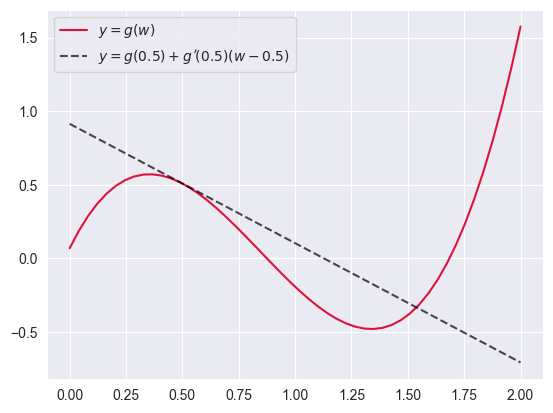
\includegraphics[width=0.35\textwidth]{../../Images/graph-and-linearapproximation.png}
    \end{multicols}

    %\centering
    %\includegraphics
\end{frame}

\begin{frame}{Second order (quadratic) approximations}
    To approximate $g$ better near $v$ (and in a larger interval around $v$), we can use the second order Taylor polynomial {--} which incorporates both first and second derivative information.  This is the function:

    \[h(w) = g(v) + g'(v)(w - v) + \frac12g''(v)(w - v)^2.\]

    
    Note: if $g'(v) = 0$ and $g''(v) > 0$, then $h(w) \ge g(v)$. So (where the approximation is quite good, sufficiently near $v$), values of the original function $g(w)$ should be larger or equal to $g(v)$ (A local minimum).

    The opposite is true if $g'(v) = 0$ and $g''(v) < 0$.
\end{frame}

\begin{frame}{Extending approximations to multiple variables}
    We may extend the first and second order approximations to the setting of multiple variables. This requires the use of the gradient where, if ${\bf w} = [w_1\ w_2\ \ldots\ w_N]^T$, then 
        \[\nabla g = [\frac{\partial g}{\partial w_1}\ \frac{\partial g}{\partial w_2}\ \ldots\ \frac{\partial g}{\partial w_N}]^T.\]
    The linear approximation is $h({\bf w}) = g({\bf v}) + \nabla g({\bf v})^T({\bf w} - {\bf v})$. (Note that this \emph{is} a linear function; its graph is a translate of the subspace of $\bb R^{N+1}$ that is normal to $[-\nabla g({\bf v})^T,\ 1]^T$, the translation is by a vector whose dot product with $[-\nabla g({\bf v})^T,\ 1]^T$ is equal to $g({\bf v}) - \nabla g({\bf v})^T{\bf v}$.)
\end{frame}

\section{Stationary points}

\begin{frame}{Stationary points versus (local) minimal}
\end{frame}

\begin{frame}{First order condition}
\end{frame}

\end{document}